\documentclass[tikz,margin=1mm]{standalone}


\begin{document}
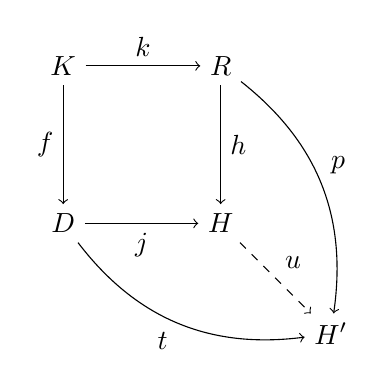
\begin{tikzpicture}[node distance=2cm, auto]
  \node (K) {$K$};
  \node[right of=K] (R) {$R$};
  \node[below of=K] (D) {$D$};
  \node[below of=R] (H) {$H$};
  \node[node distance=1.4cm, right of=H, below of=H] (H') {$H'$};

  \draw[->] (K) to node{$k$} (R);
  \draw[->] (K) to node[swap]{$f$} (D);
  \draw[->] (R) to node{$h$} (H);
  \draw[->] (D) to node[swap]{$j$} (H);

  \draw[->, bend left ] (R) to node{$p$} (H');
  \draw[->, bend right] (D) to node[swap]{$t$} (H');

  \draw[->, dashed] (H) to node{$u$} (H');

\end{tikzpicture}
\end{document}